% Universidade Aberta
% Template TeX para relatório de trabalhos
% 2025
%
%
% Dados para a capa
\newcommand{\Titulo}{Planeamento e Desenvolvimento de Sistemas de Informação}
\newcommand{\SubTitulo}{Trabalho Grupo - Topico 6}
\newcommand{\Ano}{2025}
\newcommand{\Autor}{
    Pedro Morais - 2401849 \\
    Hugo Gonçalves - 2100562 \\
    Pedro Moro - 2001642 \\
    Luis Peixoto - 2402741 \\
}
%
%
\documentclass[12pt,a4paper,final]{article}
\usepackage{csquotes}
\usepackage{float}
\usepackage[portuguese]{babel}
\usepackage{polyglossia}
\usepackage{longtable}
\setdefaultlanguage{portuguese}
\usepackage{graphicx}
\graphicspath{ {./images/} }
\usepackage[a4paper,top=3cm,bottom=3cm,left=3.5cm,right=2cm]{geometry}
\usepackage{booktabs}
\setmainfont{Times New Roman}
\defaultfontfeatures{Ligatures=TeX}
\usepackage[pdfauthor=\Autor,
    pdftitle=\Titulo,
    colorlinks=true,
    linkcolor=black,
    citecolor=black,
    bookmarksopen=true]{hyperref}
\hypersetup{colorlinks, citecolor=black, urlcolor=black}
\usepackage{bookmark}
\usepackage[style=apa, backend=biber, sortcites, url=true, language=portuguese]{biblatex}
\usepackage{fontspec}
\DeclareLanguageMapping{portuguese}{portuguese-apa}
\addbibresource{ref.bib}
\renewcommand{\baselinestretch}{1.5}
\begin{document}
    \title{\Titulo}
    \author{\Autor}
    \date{\Ano}
    \pagenumbering{gobble}
    \begin{titlepage}
        \begin{center}
            \vspace*{4cm}

            \textbf{\large UNIVERSIDADE ABERTA}

            \textbf{\large UNIVERSIDADE DE TRÁS-OS-MONTES E ALTO DOURO}

            \vspace{1cm}

            \begin{minipage}{0.4\textwidth}
                \centering
                
\includegraphics[width=0.8\textwidth]{uab}
            \end{minipage}
            \begin{minipage}{0.4\textwidth}
                \centering
                
\includegraphics[width=0.8\textwidth]{utad}
            \end{minipage}

            \vspace{1.5cm}

            \textbf{\large \Titulo}

            \textbf{\large \SubTitulo}

            \vspace{1.5cm}

            \textbf{\large \Autor}

            \vspace{2cm}

            \textbf{\large Mestrado em Engenharia Informática e Tecnologia Web}
            \vfill
            \textbf{\Ano}
        \end{center}
    \end{titlepage}
    \renewcommand{\contentsname}{Índice}
    \cleardoublepage
    \pagenumbering{roman}
    \tableofcontents
    \newpage
    \listoffigures
    \newpage
    \cleardoublepage
    \pagenumbering{arabic}

    \section{Introdução}

    Esta iniciativa insere-se na proposta de transformação de Lisboa numa \textit{Smart City}, através da revisão integral da arquitetura empresarial da Direção Municipal de Higiene Urbana (DMHU), organização vinculada à Câmara Municipal de Lisboa.
    Nos trabalhos anteriores, foram abordadas as arquiteturas de negócio, de dados e aplicacional. ~\cite{cmllisboa2019}.

    Neste trabalho, será abordada a arquitetura tecnológica (\textit{Technology Architecture}) da DMHU. No âmbito do \textit{framework} TOGAF, esta etapa visa descrever os componentes tecnológicos, como sistemas operativos, servidores, bases de dados e plataformas de virtualização, bem como as relações entre estes elementos.
    ~\cite{opengroup2025}

    O objectivo é identificar os componentes tecnológicos essenciais, minimizando a complexidade das representações.
    Foi proposto o uso do ponto de vista de infraestrutura (\textit{Infrastructure Viewpoint}), que permite representar os elementos de \textit{software} e \textit{hardware} que suportam as camadas de aplicação e informacional.
    Elementos relacionados com o negócio e os seus processos não serão representados nesta visão, por já serem
    apresentados nos trabalhos anteriores.
    ~\cite{visualparadigm2025}

    \section{Infraestrutura de Processamento \textit{As-Is} – Q11}\label{sec:infra-estrutura-de-processamento-textit{as-is}--q11}

    Nesta secção é apresentada uma visão da infraestrutura de processamento (\textit{Processing Infrastructure}) da
    DMHU. O foco recai sobre os sistemas operativos, servidores e \textit{hypervisors} em uso.
    A maioria das aplicações
    encontra-se alojada no edifício central da Câmara Municipal de Lisboa.

    Existem ainda sistemas externos, como o SAP, Cartrack e Bee2Waste, geridos pelos respetivos fornecedores e disponibilizados à DMHU via web.
    Como a infraestrutura destes sistemas não se encontra sob gestão da DMHU, serão representados apenas no domínio aplicacional.

    Uma situação intermédia é a dos dispositivos pessoais móveis, \textit{desktops} e portáteis que, apesar de não se encontrarem no edifício central, estão sob gestão da DMHU ou da própria CML. Nestes casos, são representados os sistemas operativos que podem ser utilizados nesses dispositivos.

    As comunicações entre o edifício central, os dispositivos pessoais e os sistemas externos são realizadas via web, sendo igualmente representadas nesta visão.

    Detalhes sobre a infraestrutura de processamento, como o dimensionamento da memória RAM e do CPU, podem ser consultados na descrição de cada objeto, no modelo Archimate que acompanha este relatório.

    \begin{figure}[H]
        \centering
        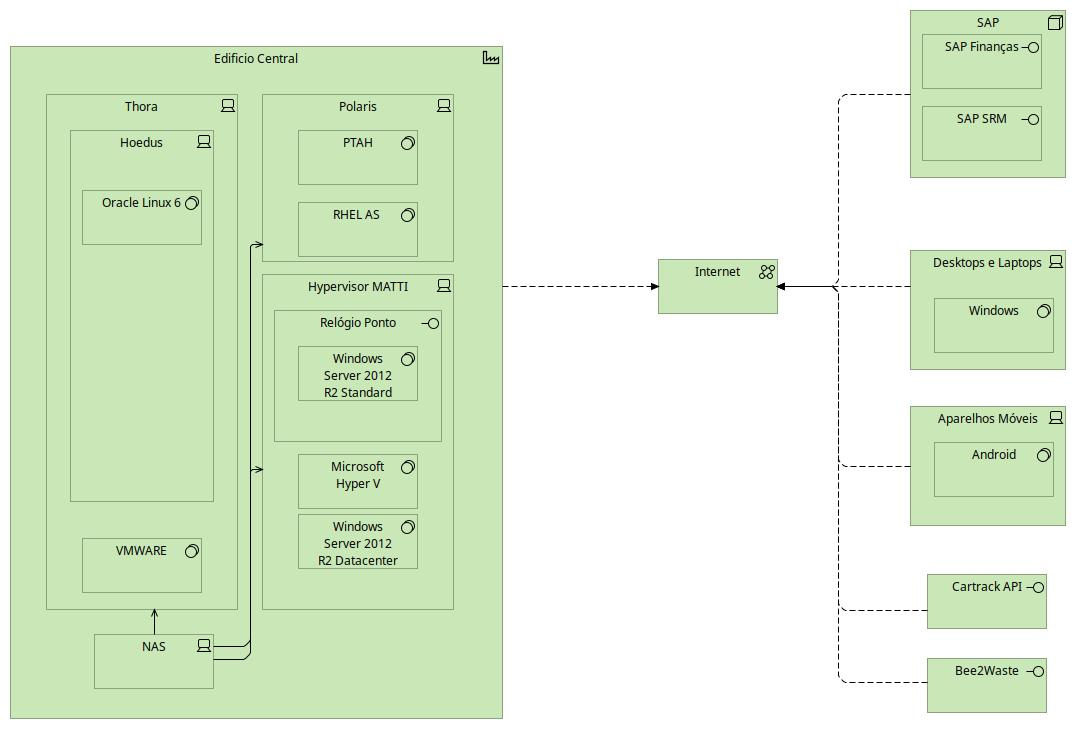
\includegraphics[width=0.9\textwidth]{Q11 - Processing Infraestructure As-Is}
        \caption{Infraestrutura de Processamento da DMHU e da CML}
        \label{fig:infra_proc}
    \end{figure}

    \section{Infraestrutura de Armazenamento \textit{As-Is} – Q12}\label{sec:infra-estrutura-de-armazenamento-textit{as-is}--q12}

    Esta secção incide sobre a infraestrutura de armazenamento das aplicações.
    O foco é dado às aplicações alojadas no edifício central, sendo excluídos os sistemas externos (cuja infraestrutura não é gerida pela CML/DMHU) e os dispositivos pessoais (com grande diversidade de capacidades de armazenamento).

    Detalhes sobre a capacidade de armazenamento encontram-se na descrição de cada objeto no modelo Archimate incluído neste relatório.

    \begin{figure}[H]
        \centering
        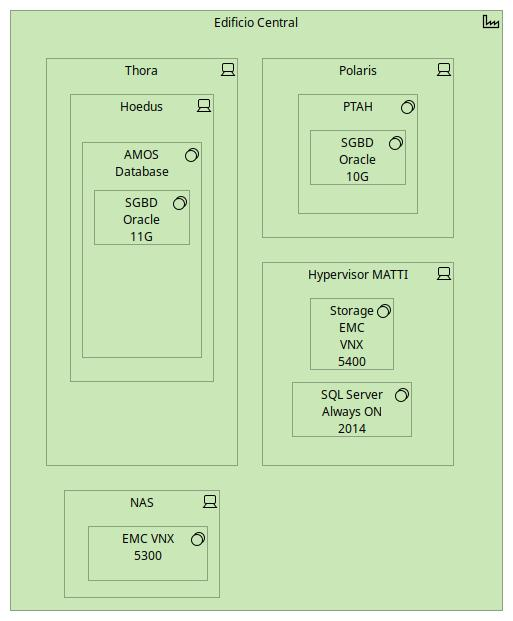
\includegraphics[width=0.9\textwidth]{Q12 - Storage Infraestructure As-Is}
        \caption{Infraestrutura de Armazenamento das aplicações alojadas no edifício central da DMHU/CML}
        \label{fig:infra_storage}
    \end{figure}

    \section{Conclusão}\label{sec:conclusao}

    Verifica-se que a CML, e consequentemente a DMHU, possui uma arquitetura maioritariamente \textit{on-premises}, concentrando os seus sistemas em infraestrutura própria localizada no edifício central.
    Esta abordagem permite um maior controlo sobre as aplicações, evitando dependência externa, mas exige investimento contínuo na manutenção das infraestruturas.

    É de salientar o uso de sistemas operativos legados, como o Windows Server, que deixou de ter suporte oficial
    pela Microsoft, tornando a arquitetura vulnerável a falhas e ataques, dada a ausência de atualizações de
    segurança. ~\cite{microsoft2023}

    Verifica-se também a utilização de sistemas operativos \textit{open source}, como o Linux, mas com distribuições proprietárias como Oracle e Red Hat (\textit{Red Hat Enterprise Linux Advanced Platform – RHEL AS}). Estas distribuições permitem uso gratuito sob certas condições, mas exigem pagamento por suporte e cargas de trabalho elevadas.
    A inclusão destas plataformas, em paralelo com as soluções baseadas em Windows, introduz alguma complexidade adicional, mas contribui para reduzir o risco de \textit{lock-in} a um único fornecedor.

    \newpage
    \printbibliography
\end{document}